Der Versuch besteht aus zwei Teilen. \\
Zunächst wird für drei verschiedene Spannungsverläufe (Rechteck, Sägezahn und Dreieck) eine \textbf{Fourier-Synthese} durchgeführt. Dazu wird ein Schwingungsgenerator benutzt, der die ersten zehn Komponenten einer Fourier-Reihe generieren kann. Es müssen jeweils die passenden Koeffizienten eingestellt und überprüft werden, dass die Schwingungen alle in Phase sind. Letzteres ist am einfachsten über Lissajous-Figuren zu bewerkstelligen. Dabei muss sich entweder (falls die Frequenzen ungerade Vielfache voneinander sind) ein Bild wie in Abbildung \ref{fig:Lissajous} zu sehen ergeben. Oder eine perfekt symmetrische liegende Acht, falls die Frequenzen gerade viele Vielfache voneinander sind. In beiden Fällen treten können auch mehr als eine \glqq Schwingung\grqq\ bzw. mehr als ein \glqq Nulldurchgang\grqq\ auftreten.
\begin{figure}[h!]
	\centering
	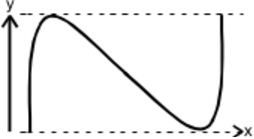
\includegraphics[width=0.25\textwidth]{Lissajous.pdf}
	\caption{Lissajous-Figur zweier in Phase schwingenden Signalen, für die gilt $\omega_1 = 3\omega_2$}
	\label{fig:Lissajous}
\end{figure} \\
Im zweiten Teil wird ein Funktionsgenerator an ein Oszilloskop angeschlossen. Mit Hilfe der \textsc{math}-Funktion des Oszilloskops wird dann eine \textbf{Fourier-Transformation} für verschiedene Spannungen (Rechteck, Sägezahn und Dreieck) durchgeführt. Nun können Ort und Amplitude der Pieks abgelesen werden. Hierbei gilt es allerdings zu beachten, dass die Frequenz, mit der die Funktion am Oszilloskop detektiert bzw. \glqq abgetastet\grqq\ wird, mindestens doppelt so groß ist, wie die größte Eingangs-Frequenz. Dieser Zusammenhang wird Abtasttheorem genannt.